\documentclass{standalone}
\usepackage{tikz}
\begin{document}
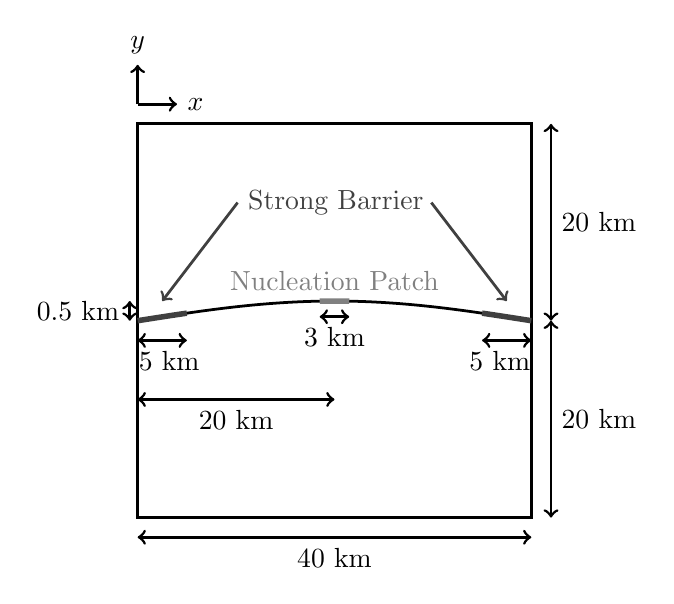
\begin{tikzpicture}[line width=1pt]
\draw (0,0) rectangle (5,5);
\draw plot[domain=0:5,smooth] (\x,{sin(\x * pi/5 r)/4.+2.5});
\draw[line width=1pt,<->] (0,-0.25) -- (2.5,-0.25) node[anchor=north]{40 km} -- (5, -0.25);
\draw[line width=1pt,<->] (5.25,0) -- (5.25,1.25) node[anchor=west]{20 km} -- (5.25, 2.5);
\draw[line width=1pt,<->] (5.25,2.5) -- (5.25,3.75) node[anchor=west]{20 km} -- (5.25, 5);
\draw[line width=2pt, color=darkgray] plot[domain=0:0.625,smooth] (\x,{sin(\x * pi/5 r)/4.+2.5});
\draw[line width=1pt,<->] (0,2.25) -- (0.4,2.25) node[anchor=north]{5 km} -- (0.625, 2.25);
\draw[line width=2pt, color=darkgray] plot[domain=4.375:5,smooth] (\x,{sin(\x * pi/5 r)/4.+2.5});
\draw[line width=1pt,<->] (4.375,2.25) -- (4.6,2.25) node[anchor=north]{5 km} -- (5, 2.25);
\draw[line width=2pt, color=gray] plot[domain=2.3125:2.6875,smooth] (\x,{sin(\x * pi/5 r)/4.+2.5});
\draw[color=gray] (2.5,2.75) node[anchor=south]{Nucleation Patch};
\draw[line width=1pt,<->] (-0.1,2.5) -- (-0.1,2.625) node[anchor=east]{0.5 km} -- (-0.1, 2.75);
\draw[line width=1pt,<->] (2.3125,2.55) -- (2.5,2.55) node[anchor=north]{3 km} -- (2.6875, 2.55);
\draw[line width=1pt,<->] (0,1.5) -- (1.25,1.5) node[anchor=north]{20 km} -- (2.5, 1.5);
\draw[line width=1pt,->] (0,5.25) -- (0.5,5.25) node[anchor=west]{$x$};
\draw[line width=1pt,->] (0,5.25) -- (0,5.75) node[anchor=south]{$y$};
\draw[line width=1pt, color=darkgray,->] (1.27,4) node[anchor=west]{Strong Barrier} -- (0.3125,2.75);
\draw[line width=1pt, color=darkgray,->] (3.73,4) -- (4.6875,2.75);
\end{tikzpicture}
\end{document}